% Created 2019-12-21 Sat 22:59
% Intended LaTeX compiler: pdflatex
\documentclass{article}
\usepackage[utf8]{inputenc}
\usepackage[T1]{fontenc}
\usepackage{graphicx}
\usepackage{grffile}
\usepackage{longtable}
\usepackage{wrapfig}
\usepackage{rotating}
\usepackage[normalem]{ulem}
\usepackage{amsmath}
\usepackage{textcomp}
\usepackage{amssymb}
\usepackage{capt-of}
\usepackage{hyperref}
\usepackage[english]{babel}
\author{Max Andric Su, Shameem Hedoo , Jack Moffat}
\bibliographystyle{plain}
\author{Jack Moffat}
\date{\today}
\title{The n-back Test}
\hypersetup{
 pdfauthor={Jack Moffat},
 pdftitle={The n-back Test},
 pdfkeywords={},
 pdfsubject={},
 pdfcreator={Emacs 27.0.50 (Org mode 9.1.9)}, 
 pdflang={English}}
\begin{document}

\maketitle
\tableofcontents


\section{Introduction}
\label{sec:org5c96cef}

In 1958, Wayne Kirchner invented the n-back test \cite{COULACOGLOU201791}. The n-back test is a visuospatial task that has been shown to improve working memory and attentional skills \cite{COLOM2013712}. The basic mechanisms of the test involve the presentation of continuous stimulis in terms of letters or pictures – for every stimulus presented, the participant has to indicate whether it matches a stimulus that was presented n stimuli ago \cite{Kane}. There are different types of n-back tests known as loads: 3-back test, 2-back test and 1-back test \cite{Forns}.

\subsection{Important Note}
\label{sec:org4f05c74}
During compilation from the .tex file, if 'unresolved citations' encountered after repeated compiling with \LaTeX{}, compile with bibtex.
(latex,latex,latex,bibtex,latex,latex works reliably)
\section{Hypothesis}
\label{sec:org7fd8c26}

Our hypothesis was that participants would have a more challenging time remembering things initially which would be reflected in a longer reaction time to congruent stimulis in the 2-back test compared to the reaction time of a 1-back test. However, as n-back tests are shown to improve working and short term memory \cite{LEONDOMINGUEZ2015167}, we expect participants to get better at remembering, reflected in shorter reaction times in responding to congruent stimulis.

\section{Materials/Methods}
\label{sec:orgcfe3467}

\subsection{Inline usage}
\label{sec:org4bd68db}
\subsubsection{R code}
\label{sec:org2d533c3}
Our results are not particularly well suited for demonstrating the capabilities of org-mode. 
The following block pulls in normative data from \cite{NormativeData} and stores it in the \textbf{tables} session
\begin{verbatim}
## install.packages('dplyr')
## install.packages('ggplot2')
## install.packages('tidyr')
library('dplyr')
library('tidyr')

d <- read.csv("./dataFromPaper/csvfpsyg-06-01544.csv")
tbl_df(d)
oneback<-slice(d,11:12)
twoback<-slice(d,18:19)
threeback<-slice(d,25:26)

mean_sd <- tbl_df(bind_rows(oneback,twoback,threeback))
rename(mean_sd,"Var"=X)
mMeanSD <- tbl_df(select(mean_sd,X:X.8,-X.2))
fMeanSD <- tbl_df(select(mean_sd,X:X.1,Girls:X.14))
mMeanSD

\end{verbatim}

Org-mode block as a function to rename columns prior to plotting
Note: Glitch wherein specifying header ``:colnames yes'' replaces the first row of table
\begin{verbatim}
newColNames <- c("n-back","M_or_SD","7","8","9","10","11","12","13")
names(df) <- newColNames
df
\end{verbatim}




\section{Results}
\label{sec:org1c8646d}

\subsection{Python Code}
\label{sec:orgcca38cd}
This code adds headers back into the data
\begin{verbatim}
import numpy as np
import pandas as pd
dArr = np.array(data)
headers = ["n-back","statistic"]
[headers.append(i) for i in range(7,14)]
headers = np.array(headers)
dArr = np.vstack((headers,dArr))

dArr
\end{verbatim}




\subsection{2 plots}
\label{sec:orgfb7e985}
Here is a plot of how improvement on various n-backs improves with age
\begin{verbatim}
import matplotlib
matplotlib.use('Agg')
import matplotlib.pyplot as plt
data=np.array(data)
datafloat=data[0:,2:].astype(np.float32)
ages=datafloat[0,:]
plt.cla()
plt.clf()
plt.plot(ages,datafloat[1,:],label=data[1,0])
plt.plot(ages,datafloat[3,:],label=data[3,0])
plt.plot(ages,datafloat[5,:],label=data[5,0])
plt.title(label="Age vs Mean Performance on various n-back tests for Adolescent Males")
plt.ylim(np.min(datafloat[5,:]),np.max(datafloat[1,:]))
plt.xlabel("Age (years)")
plt.ylabel("Mean hits")
plt.legend()
plt.savefig('./pyplot1.png')
'./pyplot1.png'

\end{verbatim}

\begin{center}
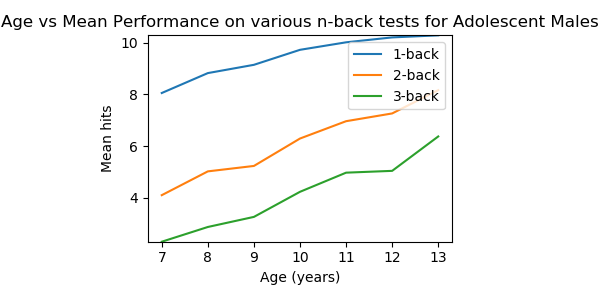
\includegraphics[width=.9\linewidth]{./pyplot1.png}
\end{center}

\begin{verbatim}
import matplotlib
matplotlib.use('Agg')
import matplotlib.pyplot as plt
data=np.array(data)
datafloat=data[0:,2:].astype(np.float32)
ages=datafloat[0,:]
plt.cla()
plt.clf()
fig=plt.figure(figsize=(6,3))
plt.errorbar(ages-0.1,datafloat[1,:],yerr=datafloat[2,:],linestyle='None',fmt='o',capsize=3,label=data[1,0])
plt.errorbar(ages,datafloat[3,:],yerr=datafloat[4,:],linestyle='None',fmt='v',capsize=3,label=data[3,0])
plt.errorbar(ages+0.1,datafloat[5,:],yerr=datafloat[6,:],linestyle='None',fmt='s',capsize=3,label=data[5,0])
plt.title(label="Age vs Mean Performance on various n-back tests for Adolescent Males, Including Error")
plt.ylim((datafloat[5,0]-datafloat[6,0]),(datafloat[0,6]+datafloat[1,6]))
plt.xlabel("Age (years)")
plt.ylabel("Mean hits")
plt.legend()
fig.tight_layout()
plt.savefig('./pyplot2.png')
'./pyplot2.png'
\end{verbatim}

\begin{center}
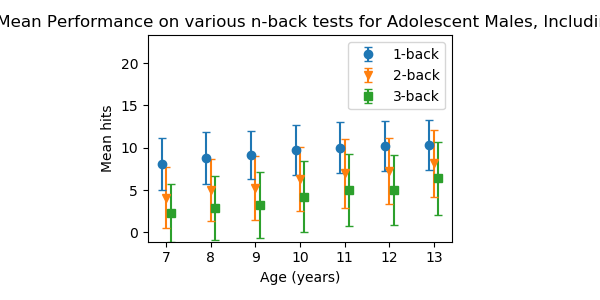
\includegraphics[width=.9\linewidth]{./pyplot2.png}
\end{center}







\section{Discussion}
\label{sec:org3460640}

Our experiment was done with the hypothesis that the reaction time to stimuli in a 1-Back test would be shorter than the reaction time to stimuli in a 2-Back test. This was based off of the fact that there is one extra letter presented between letter stimuli to remember during 2-Back tests. This test is a working memory task, but it could also potentially be used to test the recency effect, which has been shown to be eliminated when another stimulus is presented. \cite{cohen1989effects}
\section{Bibliography}
\label{sec:org3661a13}

\bibliography{references}

\section{Appendix}
\label{sec:org98e1a86}
\subsection{Python Code for n-back test}
\label{sec:org710c01e}
\begin{verbatim}
from psychopy import visual, event, core
import pandas as pd
import random
import time as systime

#########
# setup #
#############################

#############
# Make lists / define functions #
#############


def makeMatches(in_list, trials=5,
                threshold=0, n_back=2,
                keep_list_stats=True, verbose=False):
    '''Creates the matches in a given list.if a random number is greater than threshold,
    then match the letters at positions [idx] and [idx-n_back]
    in_list: list of letters, strings, etc
    trials: how many trials to run
    threshold: type(float) in range(0,1)ld
    keep_stats: Bool: will output a list with information on
    the matches (position, character) and their frequency
    verbose: Bool: prints information about the lists for immediate viewing
    '''

    # done this way to avoid changing original list, confirm necessity?
    out_list = [i for i in in_list]
    list_stats = []  # list holding the character and positions it was matched at
    num_matches = 0
    for idx, char in enumerate(in_list):
        if idx > 1:
            if (random.random() > threshold):
                out_list[idx] = in_list[idx-n_back]
                list_stats.append([(idx, idx-2), char]
                                  ) if keep_list_stats else None
                num_matches += 1

                real_match_rate = num_matches / (len(in_list) - 2)
                # show _stats or not
                if verbose:  # switch this out of a print statement for final thing so it doesnt show up
                    print(
                        f"{num_matches} of {len(in_list)-2} possible matches: {real_match_rate* 100} %")
                    print(f"in_list\n", in_list, "\nmatched list\n", out_list)
                else:
                    pass

                if keep_list_stats:
                    list_stats.insert(0, [(num_matches), "number of matches"])
                    list_stats.insert(0, [(real_match_rate), "actual match rate"])
        return(out_list, list_stats)
    else:
        return(out_list)


#####################
# create trial list #
#####################

n_trials = 15
# need to think of this inverted with how the code is currently written
match_frequency_threshold = 0.5
alphabet = [i for i in "ABCDEFGHIJKLMNOPQRSTUVWXYZ"]
initial_letters = [random.choice(alphabet) for i in range(n_trials)]

trial_list = makeMatches(initial_letters, trials=n_trials,
                         threshold=match_frequency_threshold, keep_list_stats=False)
ptt = 1.2
# ptt is the amount of time between trials, stands for "per time trial"

######################
# Window setup below #
######################
mywin = visual.Window(fullscr=True, screen=0, allowGUI=False, allowStencil=False,
                      monitor='testMonitor', color=[0, 0, 0], colorSpace='rgb')

clock = core.Clock()  # this is a clock

press_times = []  # List records the data


##############################

intro = True

if intro:
    # TODO  Find out how to display the last sentence in text_string
    text_string = f"This is an N-Back task.  This task is a test of working memory.  You will be presented with a random series of letters, one by one.  For this task, you will press the spacebar if you see a letter that was repeated two letters back.  For example, if you see a sequence such as A, D, A, then you will have to press the spacebar.  You will be given a sequence of {n_trials} letters.  "
    textList = text_string.split("  ")
    for msg in textList:
        displayMsg = visual.TextStim(
            mywin, text=msg, pos=(0.5, 0))
        mywin.flip()
        displayMsg.draw()
        core.wait(3.5)

    countdownMessage = visual.TextStim(
        mywin, text='The task will begin after this countdown.', pos=(0.5, 0))
    countdownMessage.autoDraw = True
    mywin.flip()
    core.wait(3.5)
    countdownMessage.text = ' '
    mywin.flip()
    core.wait(0.5)



countdownString = "5,4,3,2,1"
countdown = countdownString.split(',')
# ct is the countdown timer

for num in countdown:
    txtDisplay = visual.TextStim(
        mywin, text = num , alignHoriz='left', alignVert='center', pos=(0, 0))
    mywin.flip()
    txtDisplay.draw()
    core.wait(1.0)


###################
# display letters #
###################

trialTime = core.Clock()

for idx, char in enumerate(trial_list):

    trialLength = core.CountdownTimer()
    keys = event.getKeys(keyList=["space"], timeStamped = trialLength)
    txtDisplay.text = char
    mywin.flip()
    txtDisplay.draw()
    print(keys, trialLength.getTime(), txtDisplay.text)
    press_times.append([keys, trialLength.getTime(), txtDisplay.text])
    core.wait(ptt)
    txtDisplay.text = "+"
    mywin.flip()
    txtDisplay.draw()
    core.wait(ptt)
    trialLength.reset()
    # currently appending in tuple form list_stats = []  # list holding the character and positions it was matched at

endMessage = visual.TextStim(
    mywin, text = ' ', pos=(0.5, 0))
endMessage.autoDraw=True
mywin.flip()
core.wait(1.5)
endMessage.text = 'You have completed the N-Back task. Thank you!'
mywin.flip()
core.wait(3.0)

print(press_times)

ts = systime.localtime()
timestamp = str(systime.strftime("Y%yM%mD%dH%HM%MS%S",ts))
datafile = open(f"datafile_{timestamp}.txt", "w+")

################
# writing file #
################
for line in press_times:
    datafile.write(str(line))
    datafile.write("\n")
    datafile.close()

# #not sure needed
# for line in n_list:
#     datafile.write(line,)
#     datafile.write("\n")

# for line in stats:
#     datafile.write(line)
#     datafile.write("\n")

\end{verbatim}
\subsection{Example data collected from our python code}
\label{sec:org97f66f0}
The output file's name was datafile\(_{\text{Y19M12D03H16M01S43.txt}}\)
\begin{verbatim}
[[], -0.004664508000132628, 'D']
[[], -0.004164268000749871, 'Z']
[[], -0.00399026299965044, 'D']
[[], -0.0038331880004989216, 'B']
[[], -0.00503896499867551, 'Q']
[[], -0.003854009999486152, 'B']
[[], -0.0046000490001461, 'O']
[[], -0.004559805000099004, 'C']
[[], -0.003853826001432026, 'O']
[[], -0.004379994001283194, 'G']
[[], -0.0045756989984511165, 'K']
[[], -0.004432972000358859, 'E']
[[], -0.003947705999962636, 'K']
[[], -0.003957068000090658, 'D']
[[], -0.004081728999153711, 'C']
\end{verbatim}
\end{document}
